%%%%%%%%%%%%%%%%%%%%%%%%%%%%%%%%%%%%%%%%%%%%%%%%%%%%%%%%%%%%%%%%%%%
%                                                                 %
%                            CHAPTER FIVE                         %
%                                                                 %
%%%%%%%%%%%%%%%%%%%%%%%%%%%%%%%%%%%%%%%%%%%%%%%%%%%%%%%%%%%%%%%%%%%

\chapter{ANALYSIS}

\section{Model}

In the Marine Biodiversity Virtual Laboratory (MBVL) data set's case described in Section \ref{sec:MBVL}, none of these three assertions hold true. 
The process simultaneously considers all four versions so one is not transformed into another as would a sequential set of versions.
Additionally, since we do not know which version is the best, we cannot consider any data set as an update of the others.
Finally, no entity preexisted as the data sets resulted from an ongoing analysis and further steps have not been developed.

The resulting model addresses versioning by looking at the attributes of each version.
Other ontologies take a higher-level view in terms of version modeling.
While it is more specific, this implementation forces some space requirements.
PROV only requires 3 to 5 triples in order to make a versioning statement.
This model uses 9 triples for a mod change and 7 to encode addition and invalidation.
To model a version has space complexity of \(O(7M+5(A+I))\) since the version declaration statements overlap.
However, a similar structure can be achieved using \textit{prov:wasDerivedFrom} to replace modifications and \textit{schema:AddAction} and \textit{schema:DeleteAction} to replace additions and invalidations.
The resulting space complexity is \(O(7M+3A+5I)\).
This is fairly similar with additions seeing a reduction since the left-hand version no longer contributes to the \textit{schema:AddAction}.
Thus the primary benefit of using this model comes from semantics.

The reason \textit{prov:Generation} and \textit{prov:Invalidation} are not used is because they expect an activity to be responsible for an object.
However, it is not generally true that an action actively added or removed an attribute from an object in the left-hand version to produce the right-hand revision.
That assumption minimizes the ability to conduct versioning comparisons between objects that are not sequentially adjacent.
The activity producing a far away object may not immediately relate to the original data in a version comparison, resulting in a situation where it would be inappropriate to use the two PROV concepts.
When considering versioning in a state-based sense, relationships exist as a result of two objects being versions of each other.

\section{Implementation}

The versioning process breaks down to three formal steps which appear in all contexts of versioning studied in this thesis.
The first activity verifies that the objects being compared are actually versions of each other.
This exercise is often left out of details in practice since a data producer is often fairly certain as to the state of their versions.
Mechanisms are otherwise employed to enforce a strict documentation procedure to ensure the data's comparability as seen in version control software.
However, this step establishes the foundation and validity of further actions taken to version the objects.
This ensures that a mapping can be performed and will be meaningful.
The next step is generating the mapping to identify addition, invalidation, and modification relationships.
The resultant mapping in spreadsheet comparisons followed very similar rules, but when looking at the MBVL data set, the definitions were changed to achieve a specific goal.
The final step involves publishing the change information using the mapping.
In this thesis, the resulting product is published into a versioning graph.

One of the desired contributions was to study the possibility of a machine-readable change log.
In this implementation, the number of triples necessary to implement the model significantly impairs the log's ability to remain human readable.
The Noble Gas data set's change logs could not be loaded using a web browser.
One contributor to this problem is that the modification of an entire column would result in multiple entries equal to the number of rows in the table.
These entries could be combined together into a single statement relating just the effected columns.
However, this optimization would greatly impact the resulting change counts, reinforcing that version analysis depends largely on the mapping method, but this would likely allow the log to become readable.
JSON-LD proves to be a better mechanism for encoding the versioning graph than RDFa since it is intended to encode data while the latter primarily contextualizes visible content.

The advantage of this formation is that now many versions can be related together using a unified set of semantics that cannot be achieved through combining the other concepts and properties in Chapter \ref{ch:model}.
Versioning forms a continuous relationship even into later versions without introducing new semantics.
This is important since many versioning linked data alternatives view version change as a single contained activity.
When linking together multiple versions using a versioning graph, the relationship between non-adjacent editions remains implied in the graph's structure.
The natural pathway between attributes in non-adjacent versions holistically considers the relationships among all attributes along that path.
In comparison, other models only capture activity between the adjacent versions.

When considering multiple versions, a particular challenge is when an attribute does not change.
In that particular case, no links are created, but if this occurs between two transitions, the flow of change is broken.
For example, in Figure \ref{NobleGraph2}, column 31 of EGY001 becomes modified transitioning into the third version.
If that column underwent no activity in the next transition but changed from version four to five, the connection between all the column 31s would no longer be continuous.
This poses a problem for executing queries in a triple store which rely on graph traversals, but no path exists between the two modification changes in the example.

\section{Version Identification}

The versioning process discovered a discrepancy in the identifier assignment in the GCMD Keywords taxonomy.
The original analysis was intended to determine if dot-decimal identifiers could be predicted using the change counts of the versioning graph.
However, version 8.5 was named with respect to perceived taxonomy changes and did not consider underlying linked data practice revisions.
This brings into question the accuracy of all prior names and the any relationships observed between identifier and change counts.
It would explain how 8.4.1 had more additions than any previous minor change but obtains a third bracket identifier
However, assuming that the observed relationship remains, it can be shown that the keyword management team did not consider the namespace change as a major modification in their data set.
This is seen after accounting for namespace differences to show that the change count magnitude resembles other versions in the same identifier bracket.
This brings into concern the practice of version name assignment based on producer perception and not on more concrete measures.
An incomplete understanding in the amount of change between two versions can lead to flawed expectations in migrating across them.

This is not to claim that change magnitudes should be the sole mechanism in determining version identifiers.
However, it can provide a more quantitative characterization of changes within the system.
In Figure \ref{GCMDC2}, the yellow line indicates the total changes made to the data set, performing a similar function as the major/minor/revision version identifier.
However, breaking up the changes into types reveals the dominant contribution of additions to the data set.
This understanding of the data's behavior cannot be revealed with a three number dot decimal identifier system.
However, it also does not take into account the possibility that single or small changes can have significant implications scientifically.

\section{Change Analysis}

In Chapter \ref{ch:mbvl}, the versioning process was used to compare the performance of different taxonomy and algorithm combinations.
This diverges from many of the common understandings of derivations since each of the versions are not sequential and are largely independent.
The application demonstrated a case in which two data sets do not form versions.
Since they are not in a state of being revisions, implementing the version model on these two data sets would produce largely meaningless relations.
The criteria of determining valid states may seem rather dubious, and there are likely other criteria which decide more conclusively.
The data sets in this work, however, only reveal these two requirements to justify the use of versioning relationships. 

Versioning models often provide documentation on changes between versions so it is interesting applying it actively to perform analytics.
The results are able to provide a multi-lateral characterization of differences between modifications to either the choice in taxonomy or algorithm.
In order to achieve more specificity, each of the core operation concepts had to be sub-classed in order to also consider taxonomic rank.

\section{MBVL Analysis}

Figure \ref{mbvl_chart} shows the results of four comparisons performed using the matching procedure in the previous section.
There are only four comparisons because varying both taxonomy and algorithm muddles the contribution of each towards a more accurate result.
In the first set of columns, the Silva taxonomy results are versioned against RDP using the Spingo algorithm.
The naming reflects the orientation in the versioning graph so Silva forms the left-hand version and RDP would be the right-hand version.
In this comparison, using the RDP taxonomy seems to provide more accurate results, most specifically at the species level.
The taxonomies also disagree fairly often at the species and family ranks.
Switching to the Gast algorithm in the second set of columns, RDP once again demonstrates a noticeably greater accuracy in species classification.
There are also significantly fewer disagreements using the Gast algorithm between the two taxonomies.
Looking at the third set of columns, Silva demonstrates greater accuracy classifications under the Spingo algorithm than under Gast.
Over four thousand of these entries can be classified to the species level when Gast cannot.
In the fourth set of columns, RDP appears to perform better with Spingo than Gast.
However, the comparison is dominated by a much larger number of disagreements between almost six thousand entries, primarily at the species rank.
On closer inspection, this disagreement is explained by Gast classifying the species for a number of entries as unclutured bacterium.
This analysis presents evidence that using the RDP taxonomy with the Spingo algorithm will produce the most accurate classification results.

\begin{figure}
	\centering
	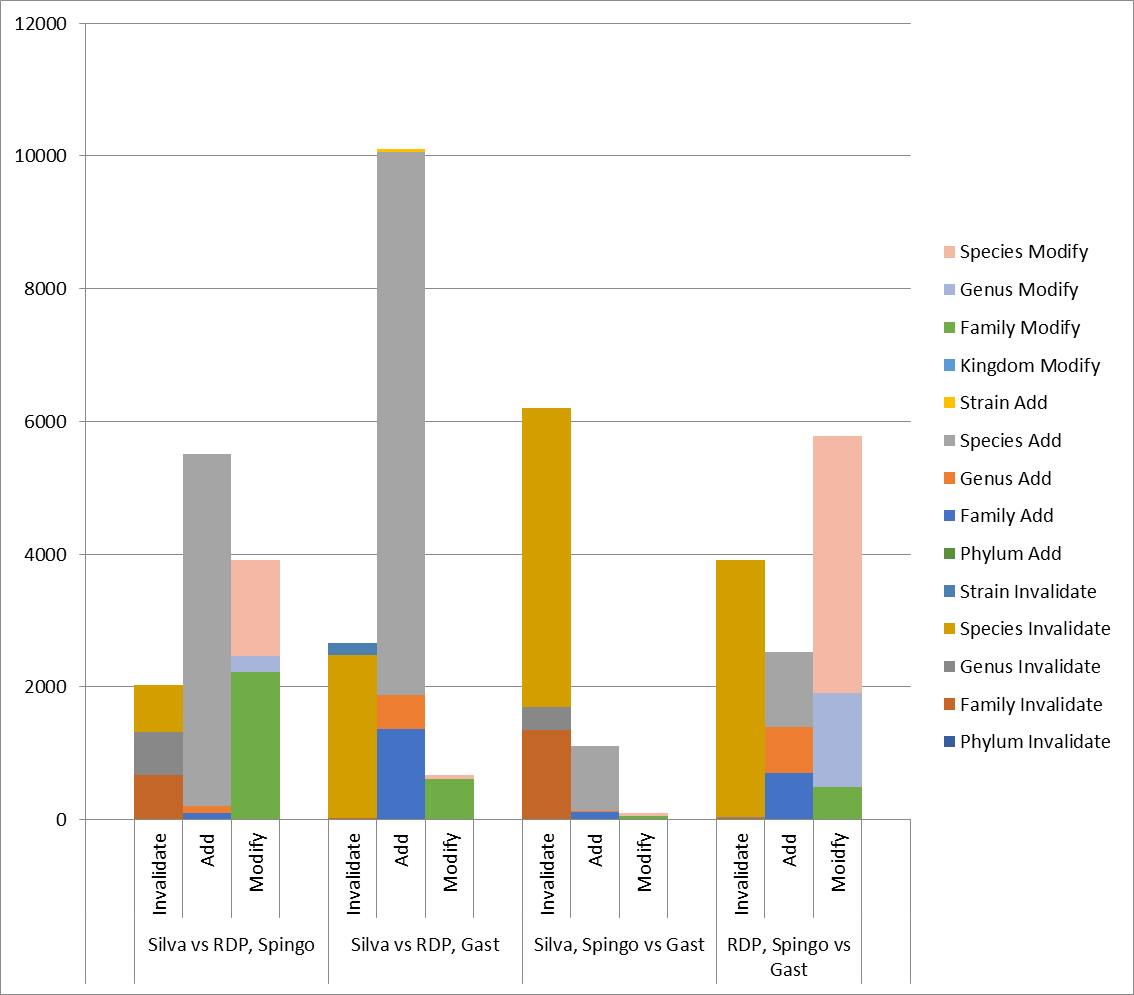
\includegraphics[scale=0.80]{figures/mbvl_chart.png}
	\caption{Compiled counts of adds, invalidates, and modifies grouped by taxonomic rank across algorithm and taxonomy combinations.}
	\label{mbvl_chart}
\end{figure}